\section{Application: Unrolling Sequential Circuits for Sequential Arithmetic Verification}
In above discussions, we propose an implicit state enumeration algorithm implemented by GB computations over
an elimination ideal, which is usually applied on FSMs working as control units. For many arithmetic
datapath components, state enumeration is not the best way to verify the function of circuit. On the one hand, the signals preloaded
to the state variables in FSM are usually not specified such that we can hardly encode the initial states; on the other
hand, instead of the set of globally reachable states, arithmetic verification focuses on exact reached states
after $k$ clock cycles which reflects desired arithmetic function. Considering these reasons, we modify
our algebraic geometry based approach and apply it to implicit FSM unrolling. 

% In above discussions, we propose an implicit state enumeration algorithm implemented by GB computation over
% an elimination ideal, which is usually applied on Mealy FSMs working as control unit. For many arithmetic
% datapath components, they should be modeled as Moore FSMs according to their structures. On the one hand, the signals preloaded
% to a Moore FSM are usually not specified such that we can hardly encode the initial states; on the other
% hand, instead of the set of globally reachable states, arithmetic verification focuses on exact reached states
% after $k$ clock cycles which reflects desired arithmetic function. Considering these reasons, we modify
% our algebraic geometry based approach and apply it to Moore FSM unrolling. 

% % Figure Moore.eps
% \begin{figure}[hbt]
% \centering{
% %\begin{minipage}{12cm}
% 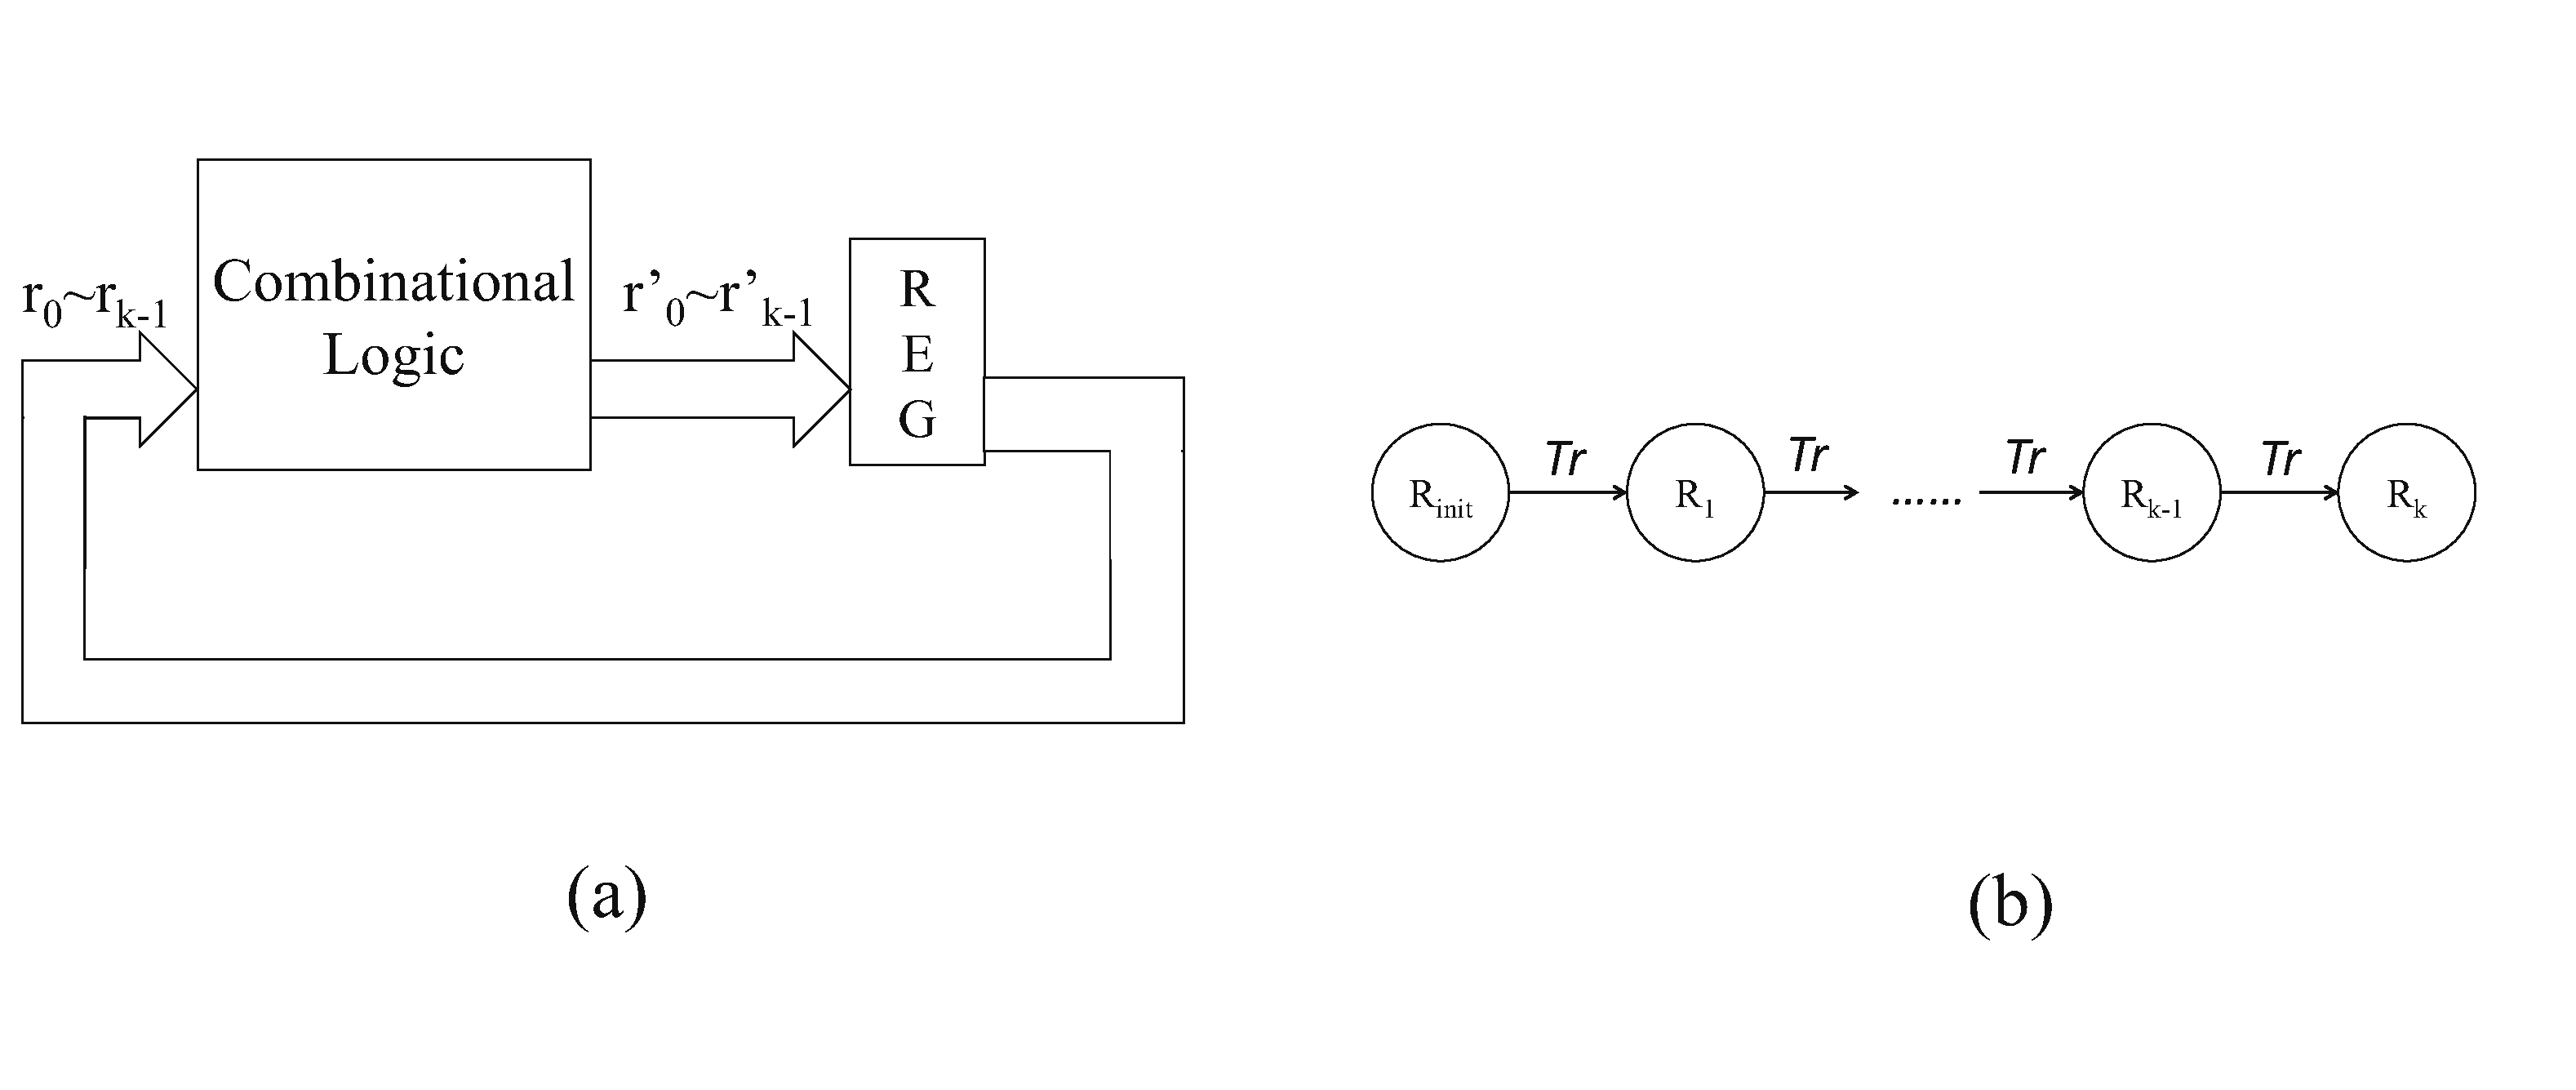
\includegraphics[width=7.5in]{./Moore.eps}
% % \vspace{-0.2in}
% \caption{A simple Moore FSM and its state transition graph}
% %\end{minipage}
% \label{fig:Moore}}
% \end{figure}

Fig.\ref{fig:seqmodel}(b) shows a typical Moore FSM without primary inputs, $R$ is the word-level state variable. Let word-level indeterminate 
$R_{init}$ denote the initial preloaded value of $R$, and $R_{i}$ denote the evaluation of $R$ after $i$ clock cycles
(transitions). Transition relation $Tr:R_{i-1}\to R_i$ can be modeled similar to
the image function in Algorithm \ref{alg:BFS}. Assume that after $k$ clock cycles, the machine should give a state output
$R_{k} = \mathcal F(R_{init})$. To verify this result, we can implicitly unroll this FSM and execute transition
function at word level for $k$ times, which is $R_{k} = Tr(R_{k-1}) = Tr(Tr(\cdots Tr(R_{init})\cdots)) = Tr^k(R_{init})$.

Sequential Galois field (GF) multiplier is a typical sequential arithmetic component widely used in cryptographic systems.
Since there is no primary input in the design, it can be regarded as Moore FSM (Fig.\ref{fig:RHmulti}(a))
where $R = \sum_{i=0}^{k-1} r_i \beta^{2^{i}}, ~A = \sum_{i=0}^{k-1} a_i
 \beta^{2^{i}}, ~B = \sum_{i=0}^{k-1} b_i \beta^{2^{i}}$. Notice that $\beta$ is the {\it normal element}
 which can be represented by a power of primitive element $\alpha:~\beta = \alpha^t$.
The states are encoded by evaluations of state variables, which can be implicitly verified 
by checking output-input function ($R = A\cdot B \pmod{P(\alpha)}$). 

% Additionally
% the inner structure of GF multiplier is XOR-rich such that we can test our approach on very large
% (>100 bits datapath) circuits.
% 
% Let us briefly describe the fundamentals behind the design of normal
% basis sequential GF multipliers, so as to put in perspective the type
% of designs that have been verified in this paper. Let $R =
% \sum_{i=0}^{k-1} r_i \beta^{2^{i}}, ~A = \sum_{i=0}^{k-1} a_i
% \beta^{2^{i}}, ~B = \sum_{i=0}^{k-1} b_i \beta^{2^{i}}$, then 
% \[
% R = A\cdot B = (\sum_{i=0}^{k-1} a_i \beta^{2^{i}}) (\sum_{j=0}^{k-1}
% b_j \beta^{2^{j}})  =
% \sum_{i=0}^{k-1}\sum_{j=0}^{k-1}a_ib_j\beta^{2^i}\beta^{2^j}\nonumber 
% \]
% 
% The expressions $\beta^{2^i}\beta^{2^j}$ are called cross-product
% terms and they can also be represented in normal basis: 
% \begin{displaymath}
% \beta^{2^i}\beta^{2^j} =
% \sum_{n=0}^{k-1}\lambda_{ij}^{(n)}\beta^{2^n}, \ \ \lambda_{ij}^{(n)}
% \in \Ftwo. 
% \end{displaymath}
% 
% From the above two equations, one can see that the expression for the
% $n^{th}$ digit of product $R = (r_0, \dots, r_n, \dots r_{k-1})$ is:
% \[
% r_n = \sum_{i=0}^{k-1}\sum_{j=0}^{k-1}\lambda_{ij}^{(n)}a_ib_j = A
% \cdot M_n \cdot B^T, ~~0 \leq n \leq k-1
% \]
% 
% where $M_n = (\lambda_{ij}^{(n)})$ is a binary $k \times k$ matrix over
% $\Ftwo$, and it is called the $\lambda$-matrix. 
%The collection of all
%$\{M_n\}$  $\lambda$-matrices is called the multiplication
%table. 
% Moreover, let $r_n = A \cdot M_n \cdot B^T$.
% Then $r_{n-1} = A \cdot M_{n-1} \cdot B^T = rotate(A) \cdot M_n
% \cdot rotate(B)^T$. This implies that $M_n$ is generated by right
% and down cyclic shifting $M_{n-1}$. Therefore, the hardware design
% of sequential GF multipliers is based on mappings of $A\cdot M_n
% \cdot B^T$ into AND-XOR gates and cyclic shift operations. 

% This paper verifies the implementation of two distinct 
% architectures of {\it sequential multipliers with parallel output
%   (SMPO)}, namely: i) the Agnew-SMPO  \cite{agnew1991implementation}
% by G. B. Agnew, which is a straight-forward implementation of the
% $\lambda$-matrix; and ii) the more recent, more complicated, yet very
% efficient RH-SMPO \cite{RHmulti}, by Reyhani-Masoleh and Hasan,
% depicted in Fig. \ref{fig:RHmulti}.  

In this proposal we use the verification of a sequential GF multiplier -- 
a 3-bit RH-SMPO invented by Reyhani-Masoleh and Hasan\cite{RHmulti} -- to illustrate our approach.
The normal element is given as $\beta = \alpha^3$, and primitive polynomial $P(\alpha) = \alpha^3+\alpha+1$.
The gate-level circuit is depicted in Fig.\ref{fig:RHmulti}(b).

\begin{figure}[hbt]
\centering{
%\begin{minipage}{12cm}
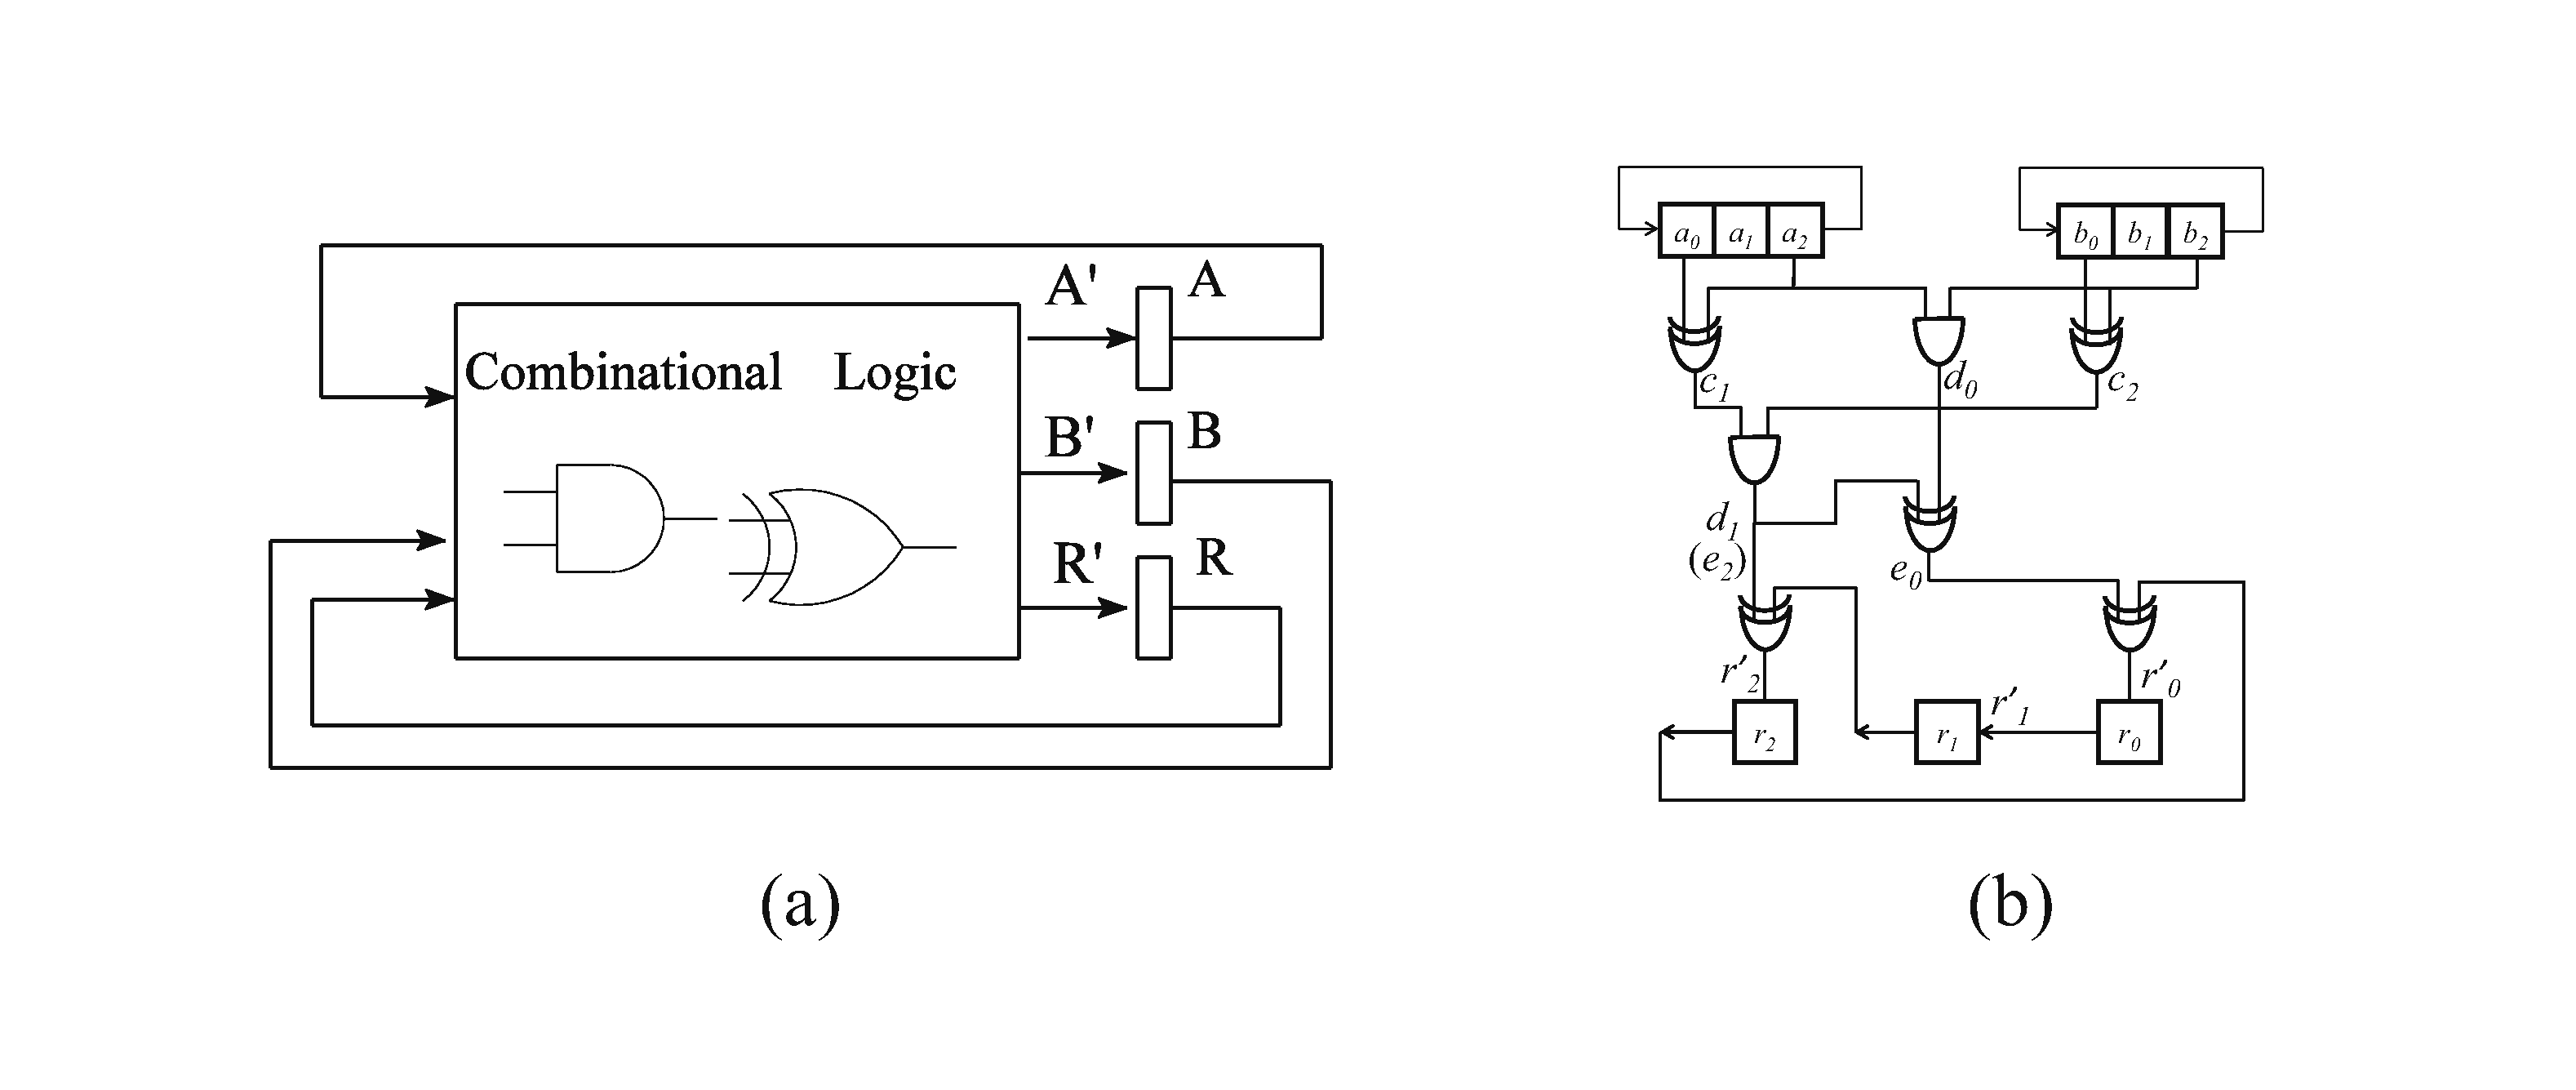
\includegraphics[width=4.5in]{./new_multi.eps}
% \vspace{-0.2in}
\caption{A 3-bit RH-SMPO and its Moore FSM model}
%\end{minipage}
\label{fig:RHmulti}}
\end{figure}

We follow  the typical sequential GF circuit model with word-level variables $A, B, R$
denoting {\it present states (PS)} and $A', B', R'$ denoting {\it next
  states (NS)} of the machine; where $A = \sum_{i=0}^{k-1} a_i \beta^{2^i}$
for the PS variables and $A' = \sum_{i=0}^{k-1} a_i'
\beta^{2^i}$ for NS variables, and so on.  Variables $R\ (R')$ correspond to those that 
store the result, and $A, B\ (A', B')$ store input operands. {\it E.g.,}
for a GF multiplier, $A_{init}, B_{init}$ (and $R_{init} =
0$) are the initial values (operands) loaded into the registers,  and
$R = \F(A_{init}, B_{init}) = A_{init} \times B_{init}$ is the final
result after $k$-cycles. Our approach aims to find this polynomial
representation for $R$.  

Each gate in the combinational logic is represented by a Boolean
polynomial. To 
this set of Boolean polynomials, we append the polynomials that define
the word-level to bit-level relations for PS and NS variables ($A =
\sum_{i=0}^{k-1} a_i \beta^{2^i}$). We denote this set of polynomials
as ideal $J = \langle 
f_1, \dots, f_s \rangle \subset \Fkk[x_1, \dots, x_d, R, R', A, A', B,
  B']$, where $x_1, \dots, x_d$ denote the bit-level (Boolean) variables
  of the circuit. The ideal of vanishing polynomials $J_0$ is also included, and
then the implicit FSM unrolling problem is setup for abstraction. 

The configurations of the flip-flops are the states of the
machine. {\it Since the set of states is a finite set of points, we
can consider it as the variety of an ideal related to the circuit
}. Moreover, since we are interested in
the {\it function encoded} by the state variables (over $k$-time
frames), we can {\it project this variety} on the word-level state
variables, starting from the initial state $A_{init}, B_{init}$.
Projection of varieties (geometry) corresponds to elimination ideals
(algebra), and can be analyzed via \Grobner bases. Therefore, we
employ a \Grobner basis computation with abstraction term order (ATO)\cite{timDAC}: we use a {\it lex term
  order} with {\it bit-level variables} 
$>$ {\it word-level NS outputs} $>$ {\it word-level PS inputs}. This
allows to eliminate all the bit-level variables 
%(corresponding to the combinational logic and the state variables),
%so as to 
and derives a representation only in terms of words. 
Consequently, $k$-successive \Grobner basis computations implicitly
unroll the machine, and provide word-level algebraic $k$-cycle
abstraction for $R'$ as $R' = \F(A_{init}, B_{init})$. 

Algorithm
\ref{alg:modified} describes our approach.  In the algorithm, $from_i$
and $to_i$ are polynomial ideals whose varieties are the valuations of
word-level variables $R, A, B$ and $R',A',B'$ in the $i$-th iteration;
and the notation ``$\setminus$'' signifies that the $NS$ in iteration
$(i)$ becomes the $PS$ in iteration $(i+1)$. Line 5 computes the Gr\"obner 
basis with the abstraction term order.  Line 6 computes the elimination 
ideal, eliminating the bit-level variables and representing the set of 
reachable states up to iteration $i$ in terms of the elimination ideal. 
These computations are analogous to those of image computations performed in FSM reachability. 
%The forward image
%$to^{i}$ is computed using \Grobner bases with ATO.

\vspace{-0.1in}
\IncMargin{1em}
\begin{algorithm}[hbt]
\SetAlgoNoLine
\LinesNumbered
 \KwIn{Circuit polynomial ideal $J$, vanishing ideal $J_0$, initial
   state ideal $R (=0), \mathcal{G}(A_{init}), \mathcal{H}(B_{init})$} 

  $from_0(R,A,B) = \langle R, \mathcal{G}(A_{init}), \mathcal{H}(B_{init})\rangle$\;
  $i = 0$\;
  \Repeat{$i == k$}
  {
  	$i \gets i + 1$\;
%	$to^i(R',A',B') \gets$  $GB( \langle J_{ckt}, J_0,
%    from^{i-1}(R,A,B)\rangle )$ with abstraction term order\;
	$G \gets$GB$( \langle J + J_0+ from_{i-1}(R,A,B) \rangle
    )$ with ATO\;
	$to_i(R',A',B')\gets G\cap \mathbb F_{2^k}[R',A',B',R,A,B]$\;
	$from_i \gets to_i(\{R,A,B\}\setminus \{R',A',B'\})$\;
  }
\Return{$from_k(R_{final})$}
\caption {Abstraction via implicit unrolling for Sequential GF circuit
  verification}
\label{alg:modified}
\end{algorithm}
\DecMargin{1em}
\vspace{-0.1in}
\begin{Example}
\label{ex:RHSMPO}

We demonstrate our approach to verify the 3-bit RH-SMPO circuit of
Fig.\ref{fig:RHmulti}. The normal element $\beta$ in
$\mathbb{F}_{2^3}$ is known to be $\beta = \alpha^3$, where $\alpha$
is the primitive element. The circuit can be described with an ideal by translating
AND and XOR gates accordingly. For the first iteration:
\begin{align*}
J = &d_0+b_2\cdot a_2,
c_1+a_0+a_2,
c_2+b_0+b_2,
d_1+c_1\cdot c_2,\\
&e_0+d_0+d_1,
e_2+d_1,
r_0'+r_2+e_0,
r_1'+r_0,
r_2'+r_1+e_2,\\
&A+a_0\alpha^3+a_1\alpha^6+a_2\alpha^{12},
B+b_0\alpha^3+b_1\alpha^6+b_2\alpha^{12},\\
&R+r_0\alpha^3+r_1\alpha^6+r_2\alpha^{12},
R'+r_0'\alpha^3+r_1'\alpha^6+r_2'\alpha^{12};
\end{align*}
The last 4 polynomials are translated from the definition of word-level variables.
This represents ideal ``$J$" from line 5 in Algorithm
\ref{alg:modified}. ``$J_0$" is the ideal of vanishing polynomials in all bit-level
variables (e.g. $a_0^2-a_0$) and word-level variables (e.g. $A^8-A$). ``$from_{i-1}$"
represents the set of current states for iteration $i$.
In the first iteration, $from_0 = \{R, A_{init}+a_0\alpha^3+a_1\alpha^6+a_2\alpha^{12},
B_{init}+b_0\alpha^3+b_1\alpha^6+b_2\alpha^{12}\}$.

After the GB computation is performed with ATO, as line 6 in Algorithm \ref{alg:modified},
we find a polynomial in variables $R', A_{init}, B_{init}$ in $to_1 : 
R'+(\alpha^2) A_{init}^4 B_{init}^4+(\alpha^2+\alpha) A_{init}^4 B_{init}^2+(\alpha^2+\alpha) A_{init}^4 B_{init}+(\alpha^2+\alpha) A_{init}^2 B_{init}^4+(\alpha^2+\alpha+1) A_{init}^2 B_{init}^2+(\alpha^2) A_{init}^2 B_{init}+(\alpha^2+\alpha) A_{init} B_{init}^4+(\alpha^2) A_{init} B_{init}^2
$.

Line 7 in Algorithm \ref{alg:modified} simply replaces NS output $R'$ with PS output
$R$ in this example; so in second iteration $from_1 = \{
R'+(\alpha^2) A_{init}^4 B_{init}^4+(\alpha^2+\alpha) A_{init}^4 B_{init}^2+(\alpha^2+\alpha) A_{init}^4 B_{init}+(\alpha^2+\alpha) A_{init}^2 B_{init}^4+(\alpha^2+\alpha+1) A_{init}^2 B_{init}^2+(\alpha^2) A_{init}^2 B_{init}+(\alpha^2+\alpha) A_{init} B_{init}^4+(\alpha^2) A_{init} B_{init}^2
, A_{init}+a_2\alpha^3+a_0\alpha^6+a_1\alpha^{12},
B_{init}+b_2\alpha^3+b_0\alpha^6+b_1\alpha^{12}\}$. 

% By continue executing the loop,
Finally, after 3 iterations we obtain: $to_3 = \{ \mathbf{R'+A_{init}B_{init},}
~A_{init}+a_0'\alpha^3+a_1'\alpha^6+a_2'\alpha^{12},
~B_{init}+b_0'\alpha^3+b_1'\alpha^6+b_2'\alpha^{12}\}$
as the image. The final result is $from_3(R_{final}) = R_{final}+A_{init}\cdot
B_{init}$, which verifies the multiplier. 
\end{Example}
Using our approach we successfully verified the function of an 100-bit RH-multiplier,
which implies its capability to handle the verification of large designs. The results
are published in \cite{myDATE}.